\documentclass{article} % For LaTeX2e
\usepackage{nips15submit_e,times}
\usepackage{hyperref}
\usepackage{url}
\usepackage{graphicx}
\usepackage{mathtools}
\usepackage{float}
\usepackage[inline]{enumitem}
\usepackage{multirow}
\usepackage[toc,page]{appendix}
\usepackage{caption} 
\captionsetup[table]{skip=10pt}
\usepackage{cite}


%\documentstyle[nips14submit_09,times,art10]{article} % For LaTeX 2.09


\title{COMPGI19 Assignment 2 Report}

\author{
Reece Doyle
\And
Navid Hallajian \\
\And
Kapileshwar Syamasundar \\
\And
Oliver Tun \\
}

\newcommand{\fix}{\marginpar{FIX}}
\newcommand{\new}{\marginpar{NEW}}

\nipsfinalcopy % Uncomment for camera-ready version

\begin{document}

\maketitle

\section{Implementation of Perceptron Algorithm}
For this problem, we implemented a perceptron trainer with the default setup; the results of our trainer and the precompiled trainer are shown in Table \ref{table:1_perf}.

\begin{table}[htb]
\centering
\caption{Classification performance for perceptron implementations}
\label{table:1_perf}
\begin{tabular}{l|l|l|}
\cline{2-3}
                                        & Our perceptron trainer & Precompiled perceptron trainer \\ \hline
\multicolumn{1}{|l|}{Average precision} & 0.5129     & 0.5262             \\ \hline
\multicolumn{1}{|l|}{Average recall}    & 0.6842     & 0.6659              \\ \hline
\multicolumn{1}{|l|}{Average F1}        & 0.5863     & 0.5879             \\ \hline
\end{tabular}
\end{table}

The results show that our trainer has lower precision and higher recall than the precompiled trainer but, overall, has roughly the same harmonic mean of the two (F1).
\section{Implementation of Average Perceptron}

Our first implementation of the averaged perceptron involved keeping a running sum of the weights used for each prediction and then, after each instance and iteration, dividing the weights by the number of predictions made. However, this naive implementation is slow because every weight (even those that have not changed) is added to the sum of weights after every prediction. In this domain, there are potentially many hundreds of thousands of features and respective weights; accessing and summing all of these weights for every training instance of every iteration is very inefficient.

Instead, we devised an alternate algorithm for accumulating the weights used for each prediction during training: for each prediction, only weights that are being changed (i.e. those associated with a candidate and the gold or predicted label) are added to the sum of weights, drastically reducing the number of weights accessed after each prediction. We achieve this by storing the last time each weight was modified so that when a weight is about to be changed, the duration of the current weight is known and can be multiplied by the weight to give the sum of that weight over the duration. This can then be added to the running sum of weights.

The results for our averaged perceptron with the default setup show it to be a lot better than the precompiled perceptron; these are shown in Table \ref{table:2_perf}.

\begin{table}[htb]
\centering
\caption{Classification performance for average perceptron implementations}
\label{table:2_perf}
\begin{tabular}{l|l|l|}
\cline{2-3}
                                        & Our average perceptron trainer & Precompiled average perceptron trainer \\ \hline
\multicolumn{1}{|l|}{Average precision} & 0.4531                       & 0.2104                    \\ \hline
\multicolumn{1}{|l|}{Average recall}    & 0.5309             & 0.5904                     \\ \hline
\multicolumn{1}{|l|}{Average F1}        & 0.4889            & 0.3103                    \\ \hline
\end{tabular}
\end{table}


\section{Feature Engineering and Evaluation}

We first consider the difference between the perceptron and Naive Bayes learning algorithms.

Generative models like Naive Bayes account for the prior probability $p(x)$ of seeing a token. Maximising this model results in maximising $\log(p(y|x)) + \log(p(x))$. In text classification, we only care about finding the most likely label for a token $p(y|x)$. Optimising for both, sacrifices higher values of $p(y|x)$ to optimise for $p(x)$, giving less accurate predictions. However, the perceptron model only optimises for $p(y|x)$ and so it is expected for this model to perform better.

For Naive Bayes, features are independent and weighted equally. This means that features should be tailored towards identifying specific labels instead of discriminating against the tokens of a certain label. Further, choosing similar features results in maximising the prior probability leading to poorer classification. We choose a distinct subset showing the best discriminative power from the features below.

We outline and motivate potential feature templates for trigger and argument classification. Where possible, concrete evidence is provided either through training set examples or highly weighted features from training. The best set of features (for both perceptron and Naive Bayes learning methods) are then presented.
Papers that provided inspiration for features have been referenced next to the feature name.

\subsection{Trigger features}

\subsubsection{Lexical}

\textbf{Stem of token.} Many events of the same label share a common stem instead of the word itself. To generalise better, we take the stem of the word. 

This feature works well to discriminate against labels. For example, when the stem is \emph{inhibit}, a low weighting is given to the token being \emph{Positive regulation}.


\textbf{POS of token.} \cite{1} Words like conjunctions are less likely to indicate events; we expect events to be verbs since they indicate an action. The highest weighted feature in this class was for tokens with POS \emph{CC} (coordinating conjunction) to have label \emph{None}, supporting our claim. 

We see that this feature performs strongest in determining whether or not a token is of label None.

\textbf{Capitalisation.} \cite{1} This feature counts the number of capital letters in the token. In addition to capturing when a candidate was the first word of a sentence, without the need for creating an extra feature template, we can also infer if the candidate was a protein.

\subsubsection{Entity-based}

\textbf{Number of proteins in sentence.} Having no proteins in the sentence makes it less likely that the sentence contains any event. Our highest weighted feature for this template was assigning a label of \emph{None} to the current token if there were no proteins in the sentence, giving evidence that our intuition is correct. However, this feature template doesn't discriminate well between events of type other than \emph{None}.

\subsubsection{Syntax-based}

\textbf{Dependencies.} \cite{4} This class of features looks at the grammatical relations between words. Dependencies are an edge between two related words \emph{head} and \emph{mod}. Experimentally only considering dependencies as a feature didn't perform well, so we also consider the POS and stem of the related dependency to our token to give more context. 

We consider features involving the mod/head, stem of the parent, dependency and POS. Here our token is the head. We consider these dependencies up to a depth of 3, meaning that if we have an edge between tokens A and B, we also consider the dependency between B and C and C and D (if they exist). An example of a well performing feature is assigning the Binding label to tokens where the edge to its associated token is prepAs (prepositional binding) and the associated token's POS is VBZ (verb, third person singular present). An example is given in Figure \ref{fig:dep_pos_mod}.

\subsubsection{Other}

\textbf{Context.} \cite{1} We capture the stems of immediately surrounding tokens. They give us a better understanding of the context in which the token is being used. In many cases, the previous token gives a clear indication of what the current token is. Our highest weighted feature for this class labels tokens as \emph{Transcription} when the previous token is \emph{mRNA}. The previous word helps limit the events that the current token can be, so it works well in discriminating between all event labels. As a result, we see that we have highly negatively weighted features as well such as assigning the label \emph{Gene expression} when the previous token is \emph{mRNA}.

Looking at the next token did not discriminate between labels as well as looking at the previous token, but it helped. An example found in the training set was assigning the label \emph{Positive regulation} when the next token has stem \emph{chromosom}.

\subsubsection{Perceptron features}
\begin{itemize*}
\item Stem of word
\item POS of word
\item Number of capital letters in word
\item Prior word
\item Next word
\item Number of proteins in sentence
\item Level 1 dependency count
\item Level 2 dependency count
\item Level 3 dependency count
\item Level 1 dependency type and POS of mod
\item Level 2 dependency type and POS of mod
\item Level 3 dependency type and POS of mod
\item Level 1 dependency type and stem of mod
\item Level 2 dependency type and stem of mod
\item Level 3 dependency type and stem of mod
\item Level 1 dependency type and stem of head
\item Level 1 dependency type and POS of head
\end{itemize*}


\subsubsection{Naive-Bayes features}
\begin{itemize*}
\item Stem of word
\item Number of capital letters in word
\item Number of proteins in sentence
\item Level 1 dependency type and POS of mod
\end{itemize*}


\subsection{Argument features}

\subsubsection{Lexical}

\textbf{POS.} These features provide semantic and contextual information related to the candidate and parent tokens. For example, \emph{Theme} arguments generally have a POS value of \emph{NN}, differentiating \emph{Theme} from \emph{Cause} and \emph{None} labels. POS values for events reveal information related to their child arguments as certain events are likely to have a specific POS related to them. Figure \ref{fig:pos_candidate_parent} shows an example of classifying \emph{Theme}.

\textbf{Value of word.} Certain argument types relate to specific sets of words so creating features based on these values helps capture this information.

\textbf{Stem.} Stem features provide a more generalised version of word features as the they group words related to a common theme. These can be useful to determine what event trigger the parent token relates to, in turn revealing information related to the argument label of the candidate.

\textbf{Capitalised letters in candidate.} \cite{3} Since some candidates have capital letters in their name, we can use the set of capitalised letters to identify proteins more accurately.

\subsubsection{Entity-based}

\textbf{Candidate is a protein.} Many of the arguments of type \emph{Cause} and \emph{Theme} are proteins. We can filter out arguments of type \emph{None} by identifying if the candidate is a protein. Figure \ref{fig:candidate_is_protein} demonstrates this.

\textbf{Number of proteins.} Following on from the last feature, if there are no proteins in a sentence, it is likely that the arguments in the sentence are of type \emph{None}. Counting the number of proteins in the sentence can capture this information.

\subsubsection{Syntax-based}

\textbf{McClosky dependency between candidate and parent.} \cite{1} In general, a specific type of McClosky dependency exists between an event and its arguments. We can use these dependencies to map to specific argument types in order to classify a candidate. Figure \ref{fig:mc_dep_candidate_parent} demonstrates this.

\textbf{Number of McClosky dependencies on candidate.} Counting the number of dependencies on the candidate can provide insight on its argument type Different argument types may have more dependencies than others. Additionally, it also recognises events that are also arguments since they are likely to have many dependencies and relationships with other tokens.

\textbf{Number of McClosky dependencies on parent.} Counting the number of dependencies on the parent can help classify which type of event it may relate to and therefore assist in classifying the candidate to a specific argument type.

\subsubsection{Other}

\textbf{Context.} This feature template refers to using the prior token as described in trigger features, including considering its stem (as a more general case of using the full prior word) and its POS value to capture sentence context.

\textbf{Absolute token distance between candidate and parent.} \cite{2} We observed that arguments are often located close to their parent token, meaning that bounds can be set to filter out arguments of type \emph{None}. Upon further inspection, most distances above the value of 40 tended to be arguments of type \emph{None}. As a result, the value was used as a cut-off point to classify \emph{None} tokens.

\textbf{Candidate POS is \emph{NN} and is a protein.} From observation, there were many cases where a \emph{Theme} argument had the POS value \emph{NN} and was also a protein. Figure \ref{candidate_nn_protein} demonstrates this.

\subsubsection{Perceptron features}

\begin{itemize*}

\item POS of candidate and parent are equivalent
\item POS of candidate and parent
\item Stem of candidate and parent
\item Stem of parent and candidate is protein
\item Candidate is protein and has capital letter
\item Number of proteins in sentence
\item Candidate is protein
\item Dependency from candidate to parent
\item Dependency from parent to candidate
\item Stem of prior word and candidate
\item POS of prior word and candidate
\item Absolute distance (number of tokens) between candidate and parent

\end{itemize*}

\subsubsection{Naive-Bayes features}

\begin{itemize*}

\item POS of candidate and candidate is protein
\item POS of candidate and parent are equivalent
\item Candidate is protein and has capital letter
\item McClosky dependency between candidate and parent
\item Absolute distance (number of tokens) between candidate and parent
\item Number of proteins in sentence $> 0$
\item Prior POS of candidate

\end{itemize*}

\subsection{Results}

\begin{table}[hbt]
\centering
\caption{Trigger classification results}
\label{trigger_results_3}
\begin{tabular}{|l|l|l|l|l|}
\hline
Learning algorithm & Feature set used & Average precision & Average recall & Average F1 \\ \hline
Perceptron         & Perceptron       & 0.1940            & 0.8132         & 0.3133     \\ \hline
Naive Bayes        & Perceptron       & 0.0142            & 0.1323         & 0.0256     \\ \hline
Naive Bayes        & Naive Bayes      & 0.1609            & 0.7500         & 0.2650     \\ \hline
\end{tabular}
\end{table}

\begin{table}[hbt]
	\centering
	\caption{Argument classification results}
	\label{argument_results_3}
	\begin{tabular}{|l|l|l|l|l|}
		\hline
		Learning algorithm & Feature set used & Average precision & Average recall & Average F1 \\ \hline
		Perceptron         & Perceptron       & 0.07338           & 0.8675         & 0.1353     \\ \hline
		Naive Bayes        & Perceptron       & 0.01311           & 0.9066         & 0.02585    \\ \hline
		Naive              & Naive Bayes      & 0.06565           & 0.6635         & 0.1195     \\ \hline
	\end{tabular}
\end{table}

During trigger classification, when training on the perceptron we first implemented lexical features, yielding an average F1 score of 0.1237. Adding entity features increased the score to 0.1735. Addition of syntax features increased the score to 0.2540 and other features raised the score to 0.3133. As shown in Table \ref{trigger_results_3}, using these features on the Naive Bayes model significantly lowered the score and so a separate feature set was engineered for this. 

During argument classification, when training with the perceptron lexical features alone yielded an F1 score of 0.0375. Adding entity features improved the score to 0.0494 and addition of syntactic features raised the score to 0.0628. Finally, adding other features raised the score to 0.1353. As with triggers, a separate set of features were needed when running on the Naive Bayes model. Results for these are shown in Table \ref{argument_results_3}.

From these results we found that in all performance aspects, the perceptron model was the best learning algorithm for both classification tasks (as expected).
\section{Joint Perceptron}

\subsection{Unconstrained joint model}
The joint classifier classifies arguments and triggers together. This means that the output of the classifier's prediction function is a tuple that contains the best choice of labels (as dictated by the weights from training) for the trigger and its arguments. This can be represented as a sum of the score for the event trigger and the scores for its arguments. As the score for the triggers and arguments is dependent on their labels, maximising the overall score corresponds to finding the best labels. 

Because the unconstrained model is such that the label assigned to a trigger is independent to the labels assigned to its arguments, maximising the total score is equivalent to individually maximising the trigger and argument scores. So given a candidate, the relevant feature vector, weights and a set of possible labels for the candidate, we can define a generic argmax routine to return the most likely label. The pseudocode for such an argmax algorithm is shown below:

\begin{verbatim}
argmax(labels, candidate, weights, feat):
  scores = []
  for (elem in labels):
   featureVector = feat(candidate, elem) // create feature Vector
   score = dot(weights, featureVector)       
   scores.append((score, elem))

   // return the label of the score with highest score value
   return maxBy(scores.elem).label 
\end{verbatim}

\subsection{Constrained joint model}
As with the unconstrained version of the joint model, the scores are calculated for each trigger label and then for the argument labels for each argument. These are summed to give the overall scores for the joint structure.

For the constrained version of the joint model, the score for each trigger label is calculated and stored (rather than just storing the score of the label that maximises the score for the trigger). Then for each trigger label, the argument labels are predicted with the required constraints in place.

Two of the constraints, \emph{``A trigger can only have arguments if its own label is not None"} and \emph{``Only regulation events can have Cause arguments"} are enforced by removing illegal argument labels from the set of possible argument labels. For example, when the trigger label is \emph{None}, the arguments labels \emph{Theme} and \emph{Cause} are removed from the set of legal argument labels. These legal argument labels are the ones used to calculate the argmax of the arguments.

For each argument, the final constraint 
\emph{``A trigger with a label other than None must have at least one Theme"} is implemented by calculating the score of it being \emph{Theme} plus the maximum score of the other arguments given the available labels. The maximum score of these is then summed with the score of the trigger and the trigger and argument labels that give the maximum of these trigger-argument combined scores is returned as the argmax for this joint constrained model.

This method of implementing the constraints is a lot more efficient than calculating all possible combinations of arguments and their scores for each label and then filtering out those that violate the constraints before returning the label combination with the maximum score.

\begin{verbatim}
argmax(triggerLabels, argLabels, x):
  
  for (tlabel in triggerLabels):
    triggerScore(tlabel) = score(x, tlabel)
    if (tlabel is "None") {
      currentArgLabels = argLabels - "Theme" - "Cause"
    }
    else if (tlabel is not a regulation event label) {
      currentArgLabels = argLabels - "Cause"
    }
    else {
      currentArgLabels = argLabels
    }
  
  for (arg in x.arguments):
    argScore(arg) = score(arg, "Theme") + ...
        sum(maxScore(x.arguments != arg))
    totalScore(tlabel) = triggerScore(tlabel) + max(argScore)
    return max(totalScore).labels
\end{verbatim}

\section{Implementation and Evaluation for Problem 4}

Using the default split of 80\% training data and 20\% development data from 500 documents, we trained the per-task models from Problem 3 and the two joint models from Problem 4 over the default number of iterations, 10.

\begin{table}[htb]
\centering
\caption{Performance of models}
\label{table:all_perf}
\resizebox{\textwidth}{!}{%
\begin{tabular}{|c|l|l|l|l|}
\hline
\multicolumn{1}{|l|}{Candidate} & Metric            & Per-task Models & Unconstrained Joint Model & Constrained Joint Model \\ \hline
\multirow{3}{*}{Trigger}        & Average precision & 0.1940          & 0.1806                    & 0.2729                  \\ \cline{2-5} 
                                & Average recall    & 0.8132          & 0.8003                    & 0.7691                  \\ \cline{2-5} 
                                & Average F1        & 0.3133          & 0.2947                    & 0.4029                  \\ \hline
\multirow{3}{*}{Argument}       & Average precision & 0.07338         & 0.1362                    & 0.1864                  \\ \cline{2-5} 
                                & Average recall    & 0.8675          & 0.6330                    & 0.3880                  \\ \cline{2-5} 
                                & Average F1        & 0.1353          & 0.2242                    & 0.2518                  \\ \hline
\end{tabular}
}
\end{table}
The results in Table \ref{table:all_perf} show that the joint models improve upon the per-task models. The unconstrained joint model shows a strong improvement over the isolated argument model, with almost a doubling in average precision and a sacrifice of average recall resulting in a higher harmonic mean (F1) of the two metrics. However, the unconstrained joint model performs worse than the isolated trigger model in both precision and recall. The improved argument labelling certainly outweighs this and it is likely that this worse trigger-labelling performance is due to the perceptron algorithm penalising the trigger features in the case when the ON HOLD UNTIL UNCONSTRAINED MODEL IS UNDERSTOOD

\section{Error Analysis}
\subsection{Best performing model}
Overall we found our best model to be the joint constrained model, trained on the perceptron learning algorithm. The performance metrics we valued the highest when choosing our best model were precision and harmonic mean. While recall scores indicated a measure of completeness (quantity), we opted for precision's measure of exactness (quality) as a more relevant performance indicator.

\subsection{Types of errors}
With an average precision of 0.273, all labels suffered from errors in classification. The event label with the least misclassifications was \emph{Phosphorylation}, while the model struggled with precision for \emph{Regulation} events the most. It was found that the most common types of errors (across all types of triggers) were mislabelling candidate triggers to be \emph{None}. The following sentence shows an instance of this:

\emph{Activation and expression of the nuclear factors of activated T cells, NFATp and NFATc, in human natural killer cells: regulation upon CD16 ligand binding.}

For argument classification, average precision was 0.187. As with trigger classification, it was found that the main error was misclassifying candidate arguments to be of type \emph{None}. An example instance of when this happened is shown below:

\emph{Both nuclear run-on and actinomycin D pulse experiments strongly indicate that HU regulates c-jun mRNA expression by increasing the rate of synthesis as well as stabilizing the c-jun mRNA.}

The frequency of these types of errors can be inferred from tables \ref{table:trigs_results} and \ref{table:args_results}, where the columns represent the predicted label and the rows represent the true label.

\begin{table}[htb]
\centering
\caption{Predictions vs true labels for event triggers}
\label{table:trigs_results}
\resizebox{\textwidth}{!}{%
\begin{tabular}{|l|l|l|l|l|l|l|l|l|l|l|}
\hline
Gold | Prediction   & Phosphorylation & Negative regulation & Regulation & Protein catabolism & Binding & Positive regulation & Localization & Transcription & None & Gene expression \\ \hline
Phosphorylation     & 18              & 0                   & 0          & 0                  & 0       & 0                   & 0            & 0             & 2    & 0               \\ \hline
Negative regulation & 0               & 47                  & 3          & 0                  & 0       & 6                   & 0            & 1             & 10   & 5               \\ \hline
Regulation          & 0               & 0                   & 63         & 0                  & 0       & 11                  & 1            & 0             & 13   & 3               \\ \hline
Protein catabolism  & 0               & 0                   & 0          & 10                 & 0       & 0                   & 0            & 0             & 5    & 0               \\ \hline
Binding             & 0               & 1                   & 1          & 0                  & 54      & 6                   & 0            & 0             & 11   & 7               \\ \hline
Positive regulation & 0               & 1                   & 10         & 0                  & 0       & 172                 & 0            & 0             & 32   & 13              \\ \hline
Localization        & 0               & 0                   & 0          & 0                  & 0       & 0                   & 25           & 0             & 0    & 6               \\ \hline
Transcription       & 0               & 0                   & 1          & 0                  & 0       & 0                   & 1            & 38            & 5    & 13              \\ \hline
None                & 12              & 83                  & 279        & 11                 & 174     & 564                 & 31           & 89            & 5649 & 241             \\ \hline
Gene expression     & 0               & 0                   & 0          & 0                  & 0       & 5                   & 1            & 0             & 4    & 166             \\ \hline
\end{tabular}
}
\end{table}

\begin{table}[htb]
\centering
\caption{Predictions vs true labels for argument triggers}
\label{table:args_results}
\begin{tabular}{|l|l|l|l|}
\hline
Gold | Prediction & None & Theme & Cause \\ \hline
None & 84070 & 1763 & 3 \\ \hline
Theme & 554 & 407 & 0 \\ \hline
Cause & 77 & 11 & 0 \\ \hline
\end{tabular}
\end{table}

\subsection{Error prevention ability}
In the joint models, arguments and triggers are predicted together and so classification occurs together. This idea is very useful for argument extraction as an argument is defined over multiple words (source trigger and the argument candidate itself).

So the types of error that joint models help prevent are mainly applicable to arguments where prior knowledge of the trigger label influences the labels for its corresponding arguments. For example, if it is known that the trigger is regulation, then the arguments for such a trigger can be limited to only be of label cause. 

As a result, even if the trained weights predict an illegal label, through constraints we can force classifications to a label (potentially the correct one) of a lower score.


\subsection{Unresolved errors}
Using the constrained joint model, we can resolve further errors with argument features by enforcing further constraints and heuristics (from studying the dataset) that target specific trigger labels and limit the range of legal possibilities for given argument candidates. This would primarily help resolve errors where candidates with true labels that are not \emph{None} are mislabelled as other non \emph{None} labels. However as observed by the error analysis, these instances are quite rare. 

Although the constraints lower the number of possible label combinations to predict, it does not address the problem of candidates misclassified as \emph{None}. This problem lies with the features chosen. The current features do not help to strongly discriminate between identifying candidates with label \emph{None} against other specific labels. This is why the majority of the incorrectly predicted candidates are labelled as \emph{None}. In the case of the label \emph{Cause}, it is always predicted as \emph{None}. Engineering features that capture information more relevant to specific labels (as opposed to those that are more generic to any label) are how such errors can be resolved.

Another way to potentially resolve errors could be to change from a joint to a pipeline model. In this pipeline model, triggers could be predicted labels first, then incorporated when predicting arguments. This means feature templates for arguments could access predicted parent token labels. The pipeline model would still effectively be a joint model but the constraints are implemented on a lower level instead, where they can be of a more specific and complex nature.



\newpage
\begin{appendices}
\section{Examples of trigger features}

\begin{figure}[H]
  \caption{Dependency type of POS of mod}
  \centering
    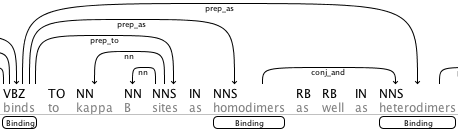
\includegraphics[width=0.75\textwidth]{images/trig_1.png}
      \label{fig:dep_pos_mod}
\end{figure}

\section{Examples of argument features}

\begin{figure}[H]
  \caption{POS of candidate and parent}
  \centering
    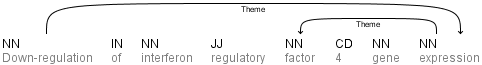
\includegraphics[width=0.75\textwidth]{images/arg_1.png}
      \label{fig:pos_candidate_parent}
\end{figure}

\begin{figure}[H]
  \caption{Candidate is a protein}
  \centering
    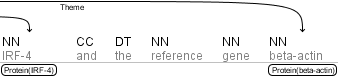
\includegraphics[width=0.75\textwidth]{images/arg_4.png}
      \label{fig:candidate_is_protein}
\end{figure}

\begin{figure}[H]
  \caption{McClosky dependency between candidate and parent}
  \centering
    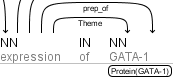
\includegraphics[width=0.30\textwidth]{images/arg_7.png}
      \label{fig:mc_dep_candidate_parent}
\end{figure}

\begin{figure}[H]
  \caption{Candidate POS is NN and is a protein}
  \centering
    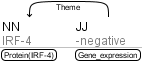
\includegraphics[width=0.30\textwidth]{images/arg_10.png}
      \label{candidate_nn_protein}
\end{figure}

\end{appendices}

\bibliography{references}{}
\bibliographystyle{plain}

\end{document}